\subsection{Descripción del algoritmo implementado.}
\vspace*{0.3cm}

La \textbf{heurística de búsqueda local} consiste en una heurística que comienza con una solución dada que intentamos mejorar. Llamaremos a esta solución ``candidata''. Luego, revisamos iterativamente sus soluciones ``vecinas''. Este conjunto de soluciones vecinas conforma el espacio de búsqueda y sus elementos son también potenciales soluciones candidatas. Esto sólo es posible si la vecindad contiene más elementos aparte de nuestra solución actual.

Si existe una mejor solución, se toma como solución actual y se repite el proceso, buscando en la vecindad de la nueva solución.

En particular, utilizamos una solución generada por la heurística golosa y verificamos mediante la búsqueda local si ésta es mejorable.

\vspace*{0.3cm}

Para nuestro algoritmo, planteamos las siguientes 2 estrategias para elegir vecindades:

\begin{itemize}
    \item \textbf{mover:} Una partición es vecina de otra si consiste en mover un único vértice de un conjunto a otro, es decir, $P$ y $Q$ son vecinas si existen $v \in A \in P$ y $B \in Q$ tales que $A - v = B$.

    \item \textbf{intercambiar:} Una partición es vecina de otra si consiste en intercambiar 2 vértices de distintos conjuntos, es decir, $P$ y $Q$ son vecinas si existen $v \in A \in P$ y $w \in B \in Q$ tales que $(A - v) \cup \{w\} = (B - w) \cup \{v\}$.
\end{itemize}

Los algoritmos consisten en, partiendo de una solución inicial, probar todas las soluciones vecinas, y continuar desde la de menor peso. Cuando no se pueda mejorar más, finaliza la ejecución.

\vspace*{0.5cm}

\textbf{Pseudocódigo con la estrategia mover:}

\vspace*{0.3cm}

\begin{verbatim}
kpmp_mover(particion) {
    pesoMin = peso(particion)
    sePuedeMejorar = true
    mientras sePuedeMejorar {
        por cada vertice en vertices(particion) {
            conjuntoDelVertice = buscarConjunto(particion, vertice)
            pesoSinVertice = peso(particion) - costo(conjuntoDelVertice, vertice)
            por cada conjunto en conjuntos(particion) excepto conjuntoDelVertice {
                peso = pesoSinVertice + costo(conjunto, vertice)
                si peso < pesoMin {
                    pesoMin = peso
                    verticeMin = vertice
                    conjuntoViejo = conjuntoDelVertice
                    conjuntoNuevo = conjunto
                }
            }
        }
        si pesoMin < peso(particion) {
            sacarVertice(conjuntoViejo, verticeMin)
            agregarVertice(conjuntoNuevo, verticeMin)
        } sino {
            sePuedeMejorar = false
        }
    }
}
\end{verbatim}

\newpage

\textbf{Pseudocódigo con la estrategia intercambiar:}

\vspace*{0.3cm}

\begin{verbatim}
kpmp_switch(particion) {
    pesoMin = peso(particion)
    sePuedeMejorar = true
    mientras sePuedeMejorar {
        por cada vertice1 en vertices(particion) {
            conjuntoDelVertice1 = buscarConjunto(particion, vertice)
            por cada vertice2 en vertices(particion) excepto que compartan conjunto {
                conjuntoDelVertice2 = buscarConjunto(particion, vertice)
                peso = peso(particion)
                    - costo(conjuntoDelVertice1, vertice1)
                    - costo(conjuntoDelVertice2, vertice2)
                    + costo(conjuntoDelVertice1, vertice2)
                    + costo(conjuntoDelVertice2, vertice1)
                si peso < pesoMin {
                    pesoMin = peso
                    verticeMin1 = vertice1
                    verticeMin2 = vertice2
                    conjuntoMin1 = conjuntoDelVertice1
                    conjuntoMin2 = conjuntoDelVertice2
                }
            }
        }
        si pesoMin < peso(particion) {
            sacarVertice(conjuntoDelVertice1, verticeMin1)
            agregarVertice(conjuntoDelVertice1, verticeMin2)
            sacarVertice(conjuntoDelVertice2, verticeMin2)
            agregarVertice(conjuntoDelVertice2, verticeMin1)
        } sino {
            sePuedeMejorar = false
        }
    }
}
\end{verbatim}



\newpage
\subsection{Análisis de complejidad del peor caso de una iteración del
            algoritmo de búsqueda local.}
\vspace*{0.3cm}

Sea $G = (V,E)$ y consideremos $n = |V|$ y $m = |E|$.

La función \texttt{buscarConjunto} recorre todos los conjuntos y en cada uno
busca, en tiempo logarítmico, el vértice dado. Esta función realiza sobre cada
conjunto $O(\log(\text{cantidad de vértices del conjunto}))$ comparaciones,
realizadas en $O(1)$. A su vez, la cantidad de elementos de cada conjunto está
acotada por $n$. Luego, la complejidad de esta función es $O(k\log(n))$, siendo
$k$ el parámetro de entrada.

\vspace*{0.3cm}

En cada iteración, el algoritmo de búsqueda local con la estrategia de
\textit{mover} comienza a recorrer cada vértice del grafo, realizando lo siguiente:
\begin{itemize}
  \item Se llama a la función \texttt{buscarConjunto}, la cual pertenece a
  $O(k\log(n))$.

  \item Por cada conjunto de la partición, se calcula el peso obtenido al
  agregarlo al conjunto, llamando a la función \texttt{costo}. Al igual que en
  la función \texttt{agregarAlDeMenosPeso} explicada en el ítem anterior, esto
  pertenece a $O(k + n)$.
\end{itemize}

Luego de recorrer cada vértice, se pueden llegar a realizar 2 llamados a
la función \texttt{costo}, que pertenece a $O(n)$.

Por lo tanto, en cada iteración del algoritmo de busqueda local, la complejidad
es $O(n (k\log(n) + k + n) + n) = O(nk\log(n) + nk + n^2 + n) = O(nk\log(n) +
n^2)$.

\vspace*{0.3cm}

En cada iteración, el algoritmo de búsqueda local con la estrategia de
intercambiar comienza a recorrer cada vértice del grafo, realizando lo siguiente:

\begin{itemize}
  \item Se llama a la función \texttt{buscarConjunto}, la cual pertenece a
  $O(k\log(n))$.

  \item Por cada uno de los otros vértices que no están en el mismo conjunto
  que el vértice actual:

  \begin{itemize}
    \item Se llama de nuevo a la función \texttt{buscarConjunto}.

    \item Se llama 4 veces a la función \texttt{costo}.
  \end{itemize}
\end{itemize}

Finalmente, se pueden llegar a realizar 4 llamados más a la función
\texttt{costo}.

Por lo tanto, en cada iteración del algoritmo de búsqueda local, la complejidad
es $O(n (k\log(n) + n (k\log(n) + k + n)) + k + n)$. Desarrollando, la
complejidad del algoritmo pertenece a $O(n^2k\log(n) + n^3)$.


\newpage \subsection{Experimentación y gráficos.}

\subsubsection{Tiempos de ejecución}

Para comparar los tiempos de ejecución generamos diversos grafos de entrada
variando sus tamaños y, además, probamos con una solución inicial completamente
random y con una generada por el algoritmo goloso.
\\

Variando la cantidad de vértices de un grafo denso (m = 3/4 n), a partir de la
solución que devuelve el algoritmo goloso. N va de 20 en 20.
\vspace*{0.5cm}

\begin{figure}[h]
  \begin{center}
    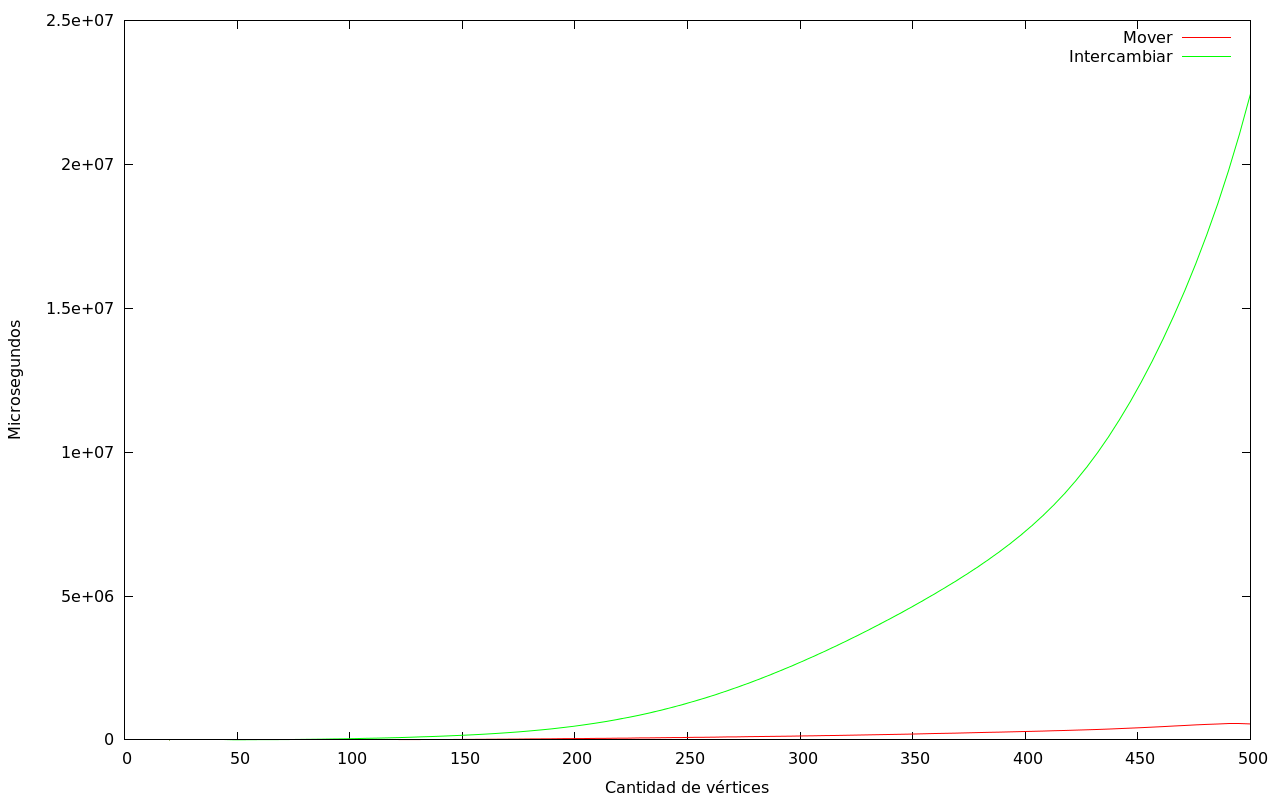
\includegraphics[scale=0.35]{imagenes/local-goloso-n-tiempo.png}
  \end{center}
\end{figure}

\vspace*{0.5cm}

Variando la cantidad de vértices de un grafo denso (m = 3/4 n), a partir de una
solución al azar. N va de 20 en 20.
\vspace*{0.5cm}

\begin{figure}[h]
  \begin{center}
    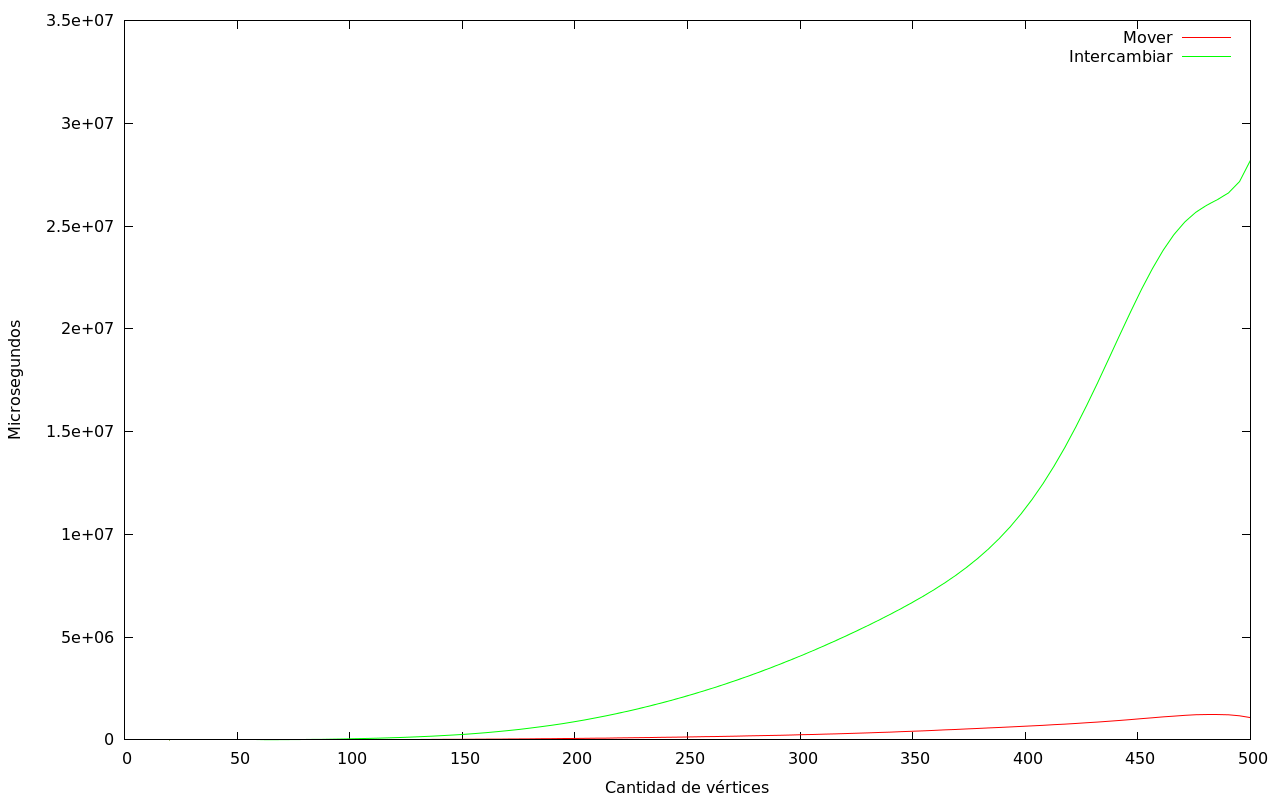
\includegraphics[scale=0.35]{imagenes/local-random-n-tiempo.png}
  \end{center}
\end{figure}

\vspace*{0.5cm}

Variando la cantidad de conjuntos de un grafo denso (n = 200, m = 150), a partir
de la solución que devuelve el algoritmo goloso. K aumenta de a 1.
\vspace*{0.5cm}

\begin{figure}[h]
  \begin{center}
    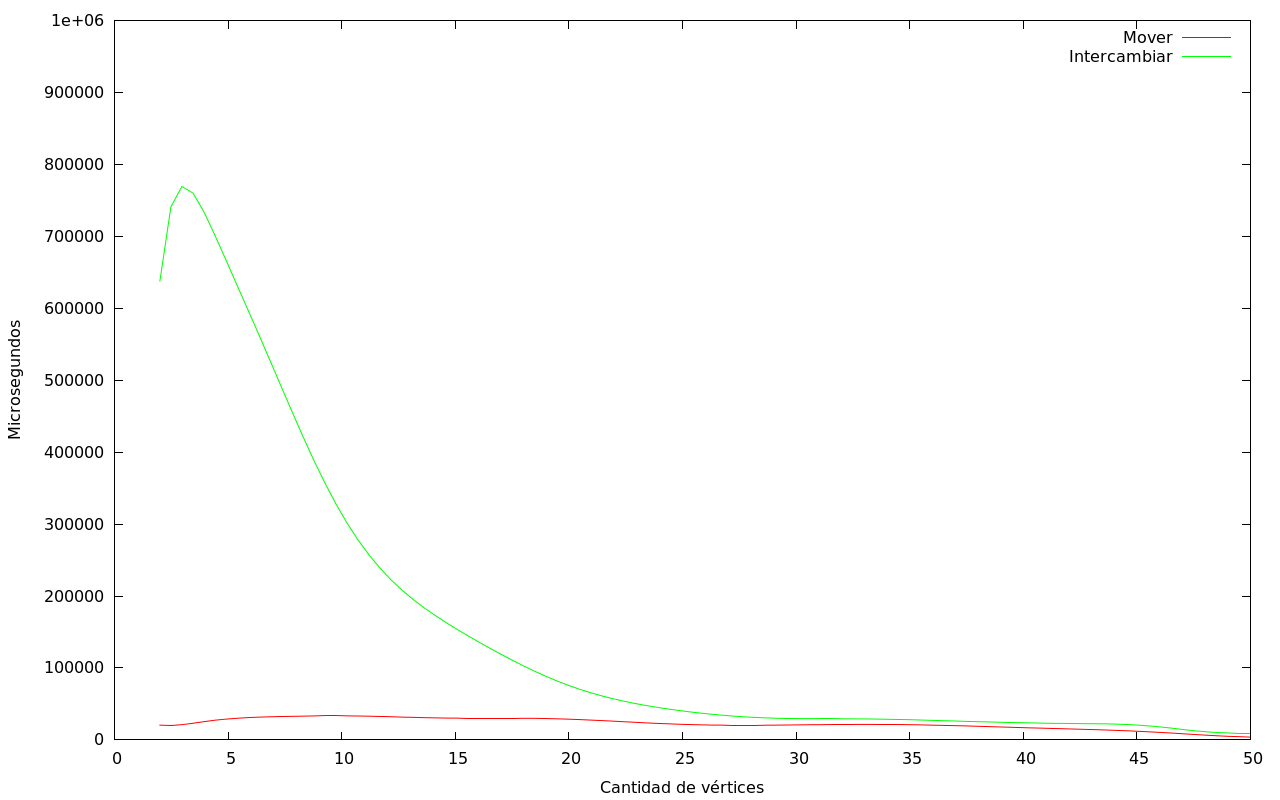
\includegraphics[scale=0.35]{imagenes/local-goloso-k-tiempo.png}
  \end{center}
\end{figure}

\vspace*{0.5cm}

Variando la cantidad de conjuntos de un grafo denso (n = 200, m = 150), a partir
de una solución al azar. K aumenta de a 1.
\vspace*{0.5cm}

\begin{figure}[h]
  \begin{center}
    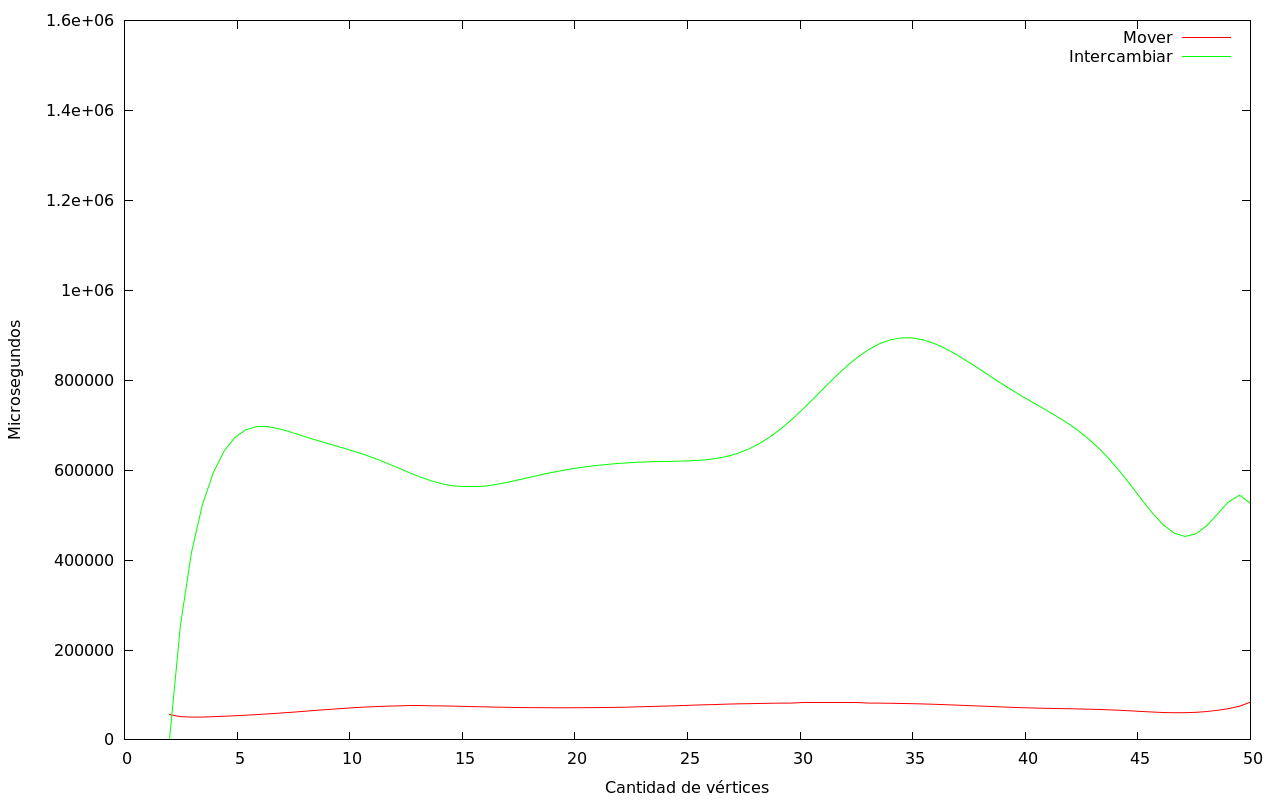
\includegraphics[scale=0.35]{imagenes/local-random-k-tiempo.png}
  \end{center}
\end{figure}

\vspace*{0.5cm}


Como puede observarse, en todos los casos el algortimo de $intercambiar$ es más
lento que el algoritmo de $mover$.

Algo que era esperable considerando que $intercambiar$ en cada iteración tiene
orden $O(n^2k\log(n) + n^3)$ vs el $O(nk\log(n) + n^2)$ de $mover$.

También se puede apreciar que el tiempo crece (en ambos casos) cuando aumenta
el $n$, también razonable ya que la complejidad depende de éste.

Sin embargo, aunque podría esperarse que también aumente ligado al $k$, con
una solución al azar, el algoritmo $mover$ se mantiene constante y el
algoritmo $intercambiar$ varía mucho, aunque también acotado. No sucede lo
mismo cuando se comienza con la solución del goloso, que se comporta
invérsamente a $k$.

Esto seguramente se deba a que, con muchos conjuntos disponible, la heurísitica
golosa da una solución muy cercana a la ideal. Luego, las heurísiticas de
búsqueda local, necesitan ejecutarse pocas veces hasta encontrar un resultado
que no puedan mejorar

\newpage \subsubsection{Calidad}

Para comparar la calidad, observamos los pesos totales de la partición
utilizando las mismas variables que para comparar los tiempos de ejecución.

Un peso menor indica una solución de mejor calidad, queremos ver si alguna
de las dos heurísticas tiene una mejor calidad consistentemente.
\\

Variando la cantidad de vértices de un grafo denso (m = 3/4 n), a partir de la
solución que devuelve el algoritmo goloso. N va de 20 en 20.
\vspace*{0.5cm}

\begin{figure}[h]
  \begin{center}
    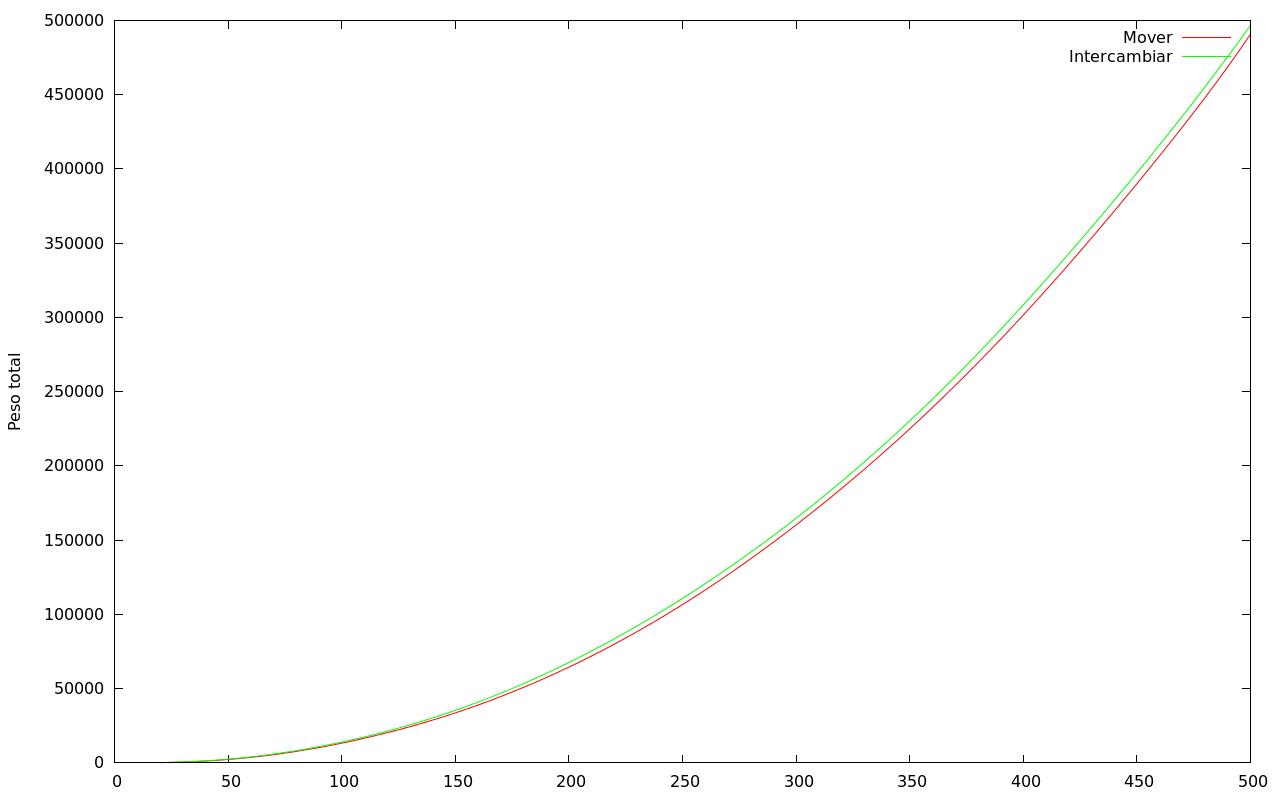
\includegraphics[scale=0.35]{imagenes/local-goloso-n-peso.png}
  \end{center}
\end{figure}

\vspace*{0.5cm}

Variando la cantidad de vértices de un grafo denso (m = 3/4 n), a partir de una
solución al azar. N va de 20 en 20.
\vspace*{0.5cm}

\begin{figure}[h]
  \begin{center}
    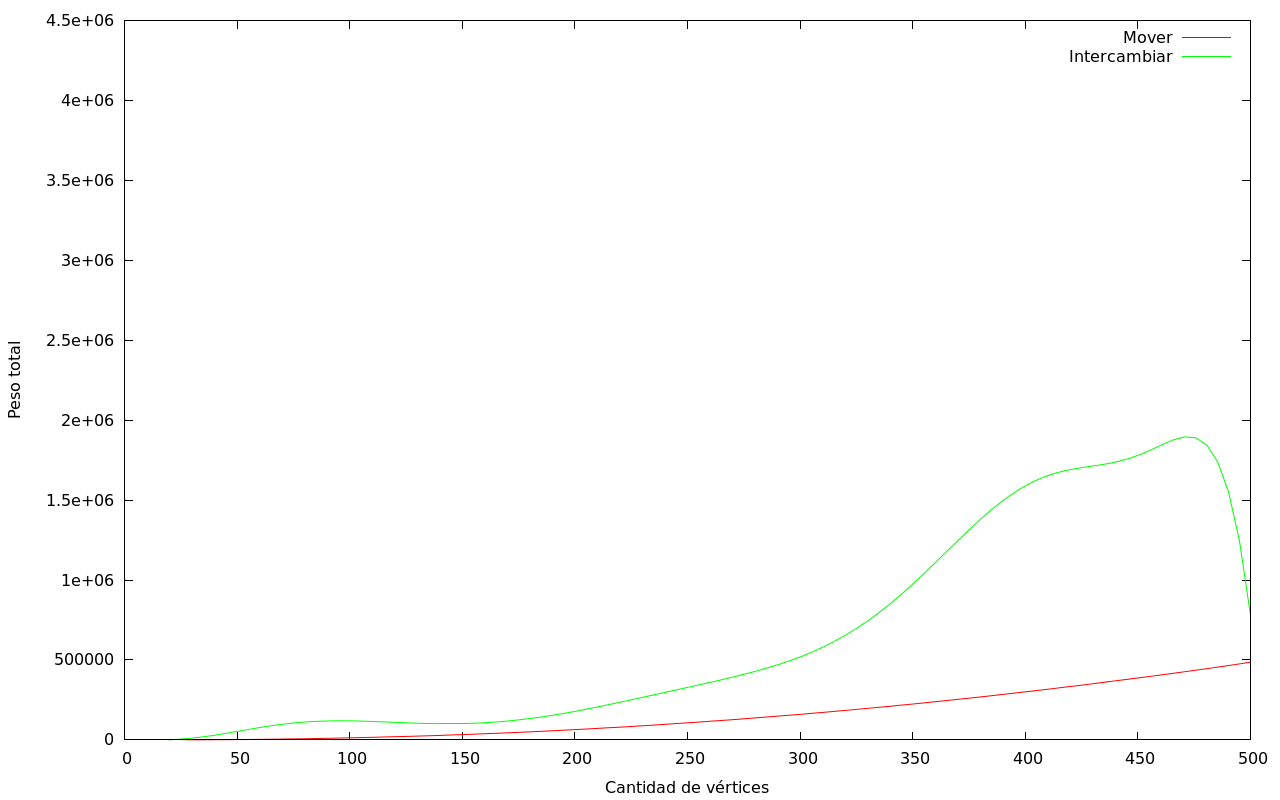
\includegraphics[scale=0.35]{imagenes/local-random-n-peso.png}
  \end{center}
\end{figure}

\vspace*{0.5cm}

Variando la cantidad de conjuntos de un grafo denso (n = 200, m = 150), a partir
de la solución que devuelve el algoritmo goloso. K aumenta de a 1.
\vspace*{0.5cm}

\begin{figure}[h]
  \begin{center}
    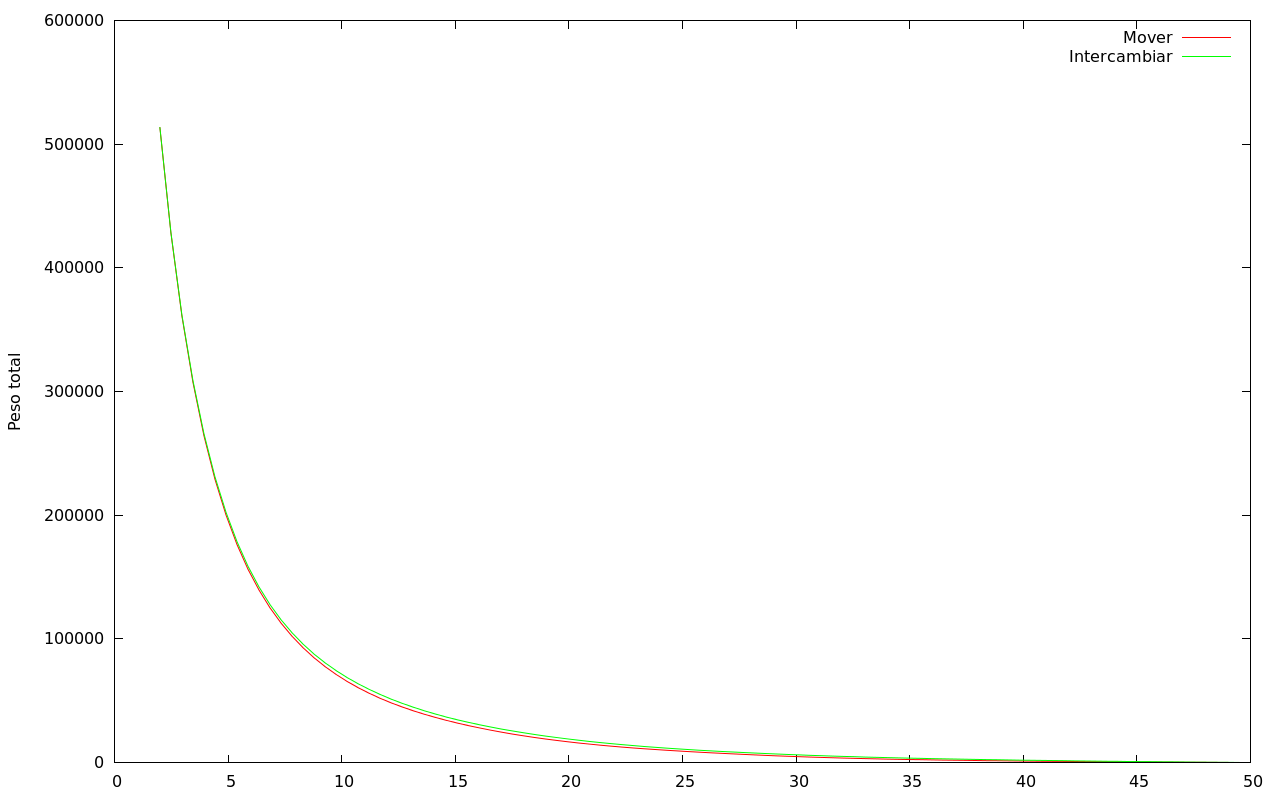
\includegraphics[scale=0.35]{imagenes/local-goloso-k-peso.png}
  \end{center}
\end{figure}

\vspace*{0.5cm}

Variando la cantidad de conjuntos de un grafo denso (n = 200, m = 150), a partir
de una solución al azar. K aumenta de a 1.
\vspace*{0.5cm}

\begin{figure}[h]
  \begin{center}
    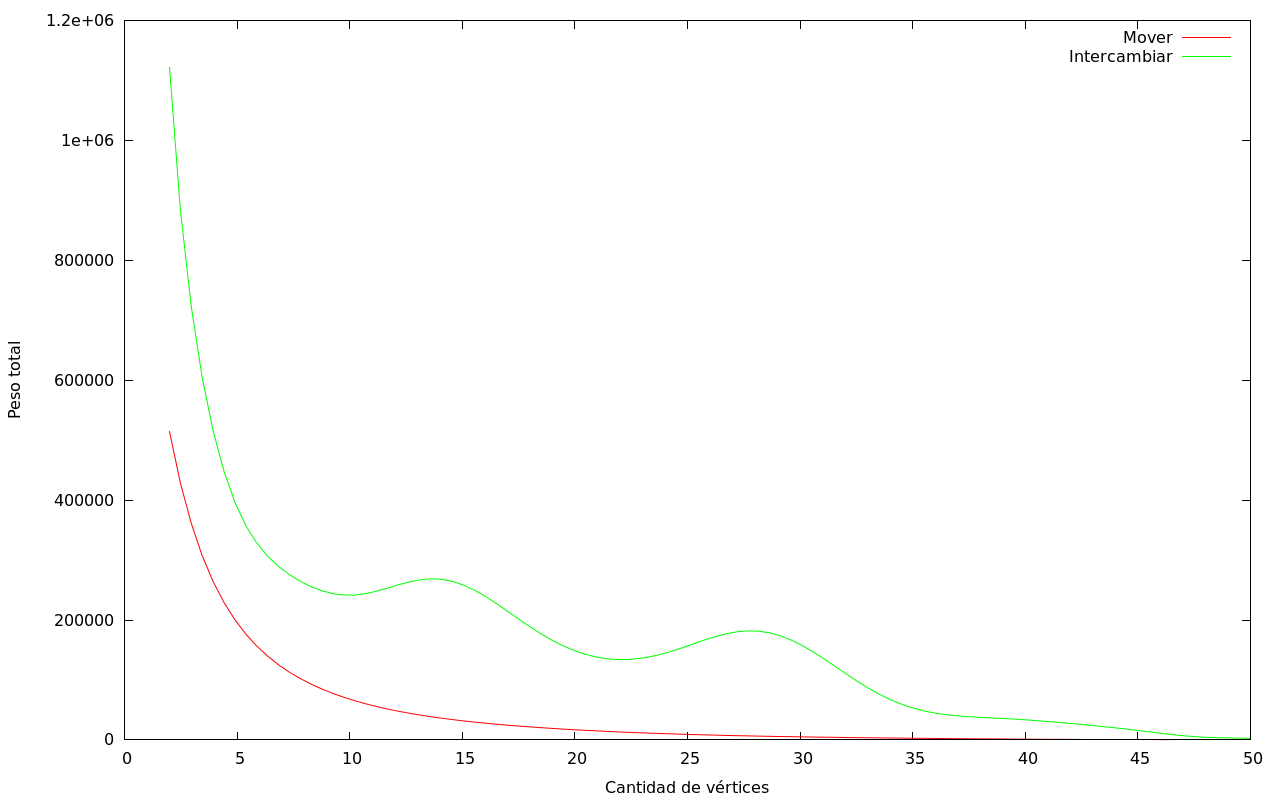
\includegraphics[scale=0.35]{imagenes/local-random-k-peso.png}
  \end{center}
\end{figure}

\vspace*{0.5cm}

Con estos gráficos se puede observar que el algoritmo $mover$ genera resultados
con mejor calidad que el algoritmo $intercambiar$ para casi todos los casos.

Variando la cantidad de vértices, el algoritmo $mover$ da resultados muy similares
empezando con la solución al azar tanto como con la solución generada por el
algoritmo goloso. Sin embargo, el algoritmo $intercambiar$ encuentra una solución
de calidad similar únicamente comenzando desde la solución del goloso.
Empezando desde la solución al azar, el peso crece mucho más rápido que el peso
del algoritmo $mover$.

Algo similar encontramos al variar la cantidad de conjuntos. Cuando se comienza
desde una solución del goloso, se comportan de forma similar. Pero empezando con
una solución aleatoria, el algoritmo $intercambiar$ no encuentra buenas soluciones
con la misma consistencia que el algoritmo $mover$.

Luego de este análisis, con mejores tiempos y mejor calidad, queda muy evidente
que conviene utilizar la heurística de búsqueda local $mover$.
